%\VignetteIndexEntry{Introduction to the EGRET package}
%\VignetteDepends{}
%\VignetteSuggests{}
%\VignetteImports{}
%\VignettePackage{}

\documentclass[a4paper,11pt]{article}

\usepackage{amsmath}
\usepackage{times}
\usepackage{hyperref}
\usepackage[numbers, round]{natbib}
\usepackage[american]{babel}
\usepackage{authblk}
\usepackage{subcaption}
\usepackage{placeins}
\usepackage{footnote}
\usepackage{tabularx}
\renewcommand\Affilfont{\itshape\small}
\usepackage{Sweave}
\renewcommand{\topfraction}{0.85}
\renewcommand{\textfraction}{0.1}
\usepackage{graphicx}

\textwidth=6.2in
\textheight=8.5in
\parskip=.3cm
\oddsidemargin=.1in
\evensidemargin=.1in
\headheight=-.3in

%------------------------------------------------------------
% newcommand
%------------------------------------------------------------
\newcommand{\scscst}{\scriptscriptstyle}
\newcommand{\scst}{\scriptstyle}
\newcommand{\Robject}[1]{{\texttt{#1}}}
\newcommand{\Rfunction}[1]{{\texttt{#1}}}
\newcommand{\Rclass}[1]{\textit{#1}}
\newcommand{\Rpackage}[1]{\textit{#1}}
\newcommand{\Rexpression}[1]{\texttt{#1}}
\newcommand{\Rmethod}[1]{{\texttt{#1}}}
\newcommand{\Rfunarg}[1]{{\texttt{#1}}}

\begin{document}
\Sconcordance{concordance:EGRET.tex:EGRET.Rnw:%
1 75 1 1 8 14 1 1 2 1 0 1 1 3 0 1 2 6 1 1 10 24 0 1 2 %
2 1 1 10 18 0 1 2 8 1 1 11 26 0 1 2 3 1 1 10 15 0 1 2 %
33 1 1 9 23 0 1 2 12 1 1 2 13 0 1 2 2 1 1 2 19 0 1 2 %
12 1 1 3 2 0 2 1 1 2 2 1 3 0 1 2 2 1 1 9 16 0 1 2 1 1 %
1 2 4 0 1 2 1 1 1 2 4 0 1 2 2 1 1 9 20 0 1 2 2 1 1 2 %
4 0 1 2 15 1 1 4 6 0 1 2 3 1 1 -5 1 9 12 1 1 2 1 0 1 %
1 3 0 1 2 2 1 1 2 1 0 1 1 3 0 1 2 4 1 1 5 1 -2 1 6 7 %
1 1 5 1 -2 1 6 8 1 1 9 4 1 1 -6 1 10 7 1 1 5 1 -2 1 6 %
15 1 1 2 4 0 1 2 3 1 1 -5 1 9 10 1 1 2 1 0 1 1 3 0 1 %
2 3 1 1 -5 1 9 9 1 1 2 4 0 1 2 3 1 1 -5 1 9 17 1 1 2 %
4 0 1 2 31 1 1 2 23 0 1 2 12 1 1 2 1 0 4 1 5 0 4 1 12 %
0 1 2 36 1 1 2 1 0 7 1 3 0 1 2 1 4 4 1 1 -6 1 10 7 1 %
1 4 1 -2 1 6 8 1 1 4 4 1 1 -6 1 10 7 1 1 4 1 -2 1 6 7 %
1 1 4 4 1 1 -6 1 10 7 1 1 4 1 -2 1 6 8 1 1 4 4 1 1 -6 %
1 10 9 1 1 2 4 0 1 2 3 1 1 -5 1 9 12 1 1 2 1 0 1 1 3 %
0 1 2 24 1 1 2 4 0 1 2 1 1 1 2 14 0 1 2 6 1 1 2 1 0 1 %
2 1 0 1 2 4 0 1 2 3 1 1 2 1 0 1 1 3 0 1 2 7 1 1 2 1 0 %
2 1 3 0 1 2 1 1 1 2 1 0 1 1 3 0 1 2 20 1}


%------------------------------------------------------------
\title{Introduction to the EGRET package}
%------------------------------------------------------------
\author[1]{Robert Hirsch}
\author[1]{Laura De Cicco}
\affil[1]{United States Geological Survey}



\maketitle
\tableofcontents

%------------------------------------------------------------
\section{Introduction to Exploration and Graphics for RivEr Trends (EGRET)}
%------------------------------------------------------------ 

For information on getting started in R, downloading and installing the package, see Appendix 1: (\ref{sec:appendix1}).

Exploration and Graphics for RivEr Trends (EGRET): An R-package for the analysis of long-term changes in water quality and streamflow. 

EGRET includes statistics and graphics for streamflow history, water quality trends, and the modeling algorithm Weighted Regressions on Time, Discharge, and Season (WRTDS). The best way to learn about the WRTDS approach and to see examples of its application to multiple large data sets is to read two journal articles.  Both are available, for free, from the journals in which they were published.

The first relates to nitrate and total phosphorus data for 9 rivers draining to Chesapeake Bay.  The URL is \cite{HirschII}: 
\url{http://onlinelibrary.wiley.com/doi/10.1111/j.1752-1688.2010.00482.x/full}

The second is an application to nitrate data for 8 monitoring sites on the Mississippi River or its major tributaries \cite{HirschIII}.  The URL is: \url{http://pubs.acs.org/doi/abs/10.1021/es201221s}

The manual available here assumes that the user understands the concepts underlying WRTDS.  Thus, reading at least the first of these papers is necessary to understanding the manual.  The method has been enhanced beyond what was published there.  The enhancement is that it now properly handles censored data by using survival regression rather than ordinary regression.  The details of that are in a manuscript currently in process by Doug Moyer and Bob Hirsch.


This vignette will walk through the major functions provided by the EGRET package. The package dataRetrieval is required for importing data in a EGRET-friendly format. The dataRetrieval package, along with download and installation instructions can be found at:
\\
\url{https://github.com/USGS-R/dataRetrieval}
\\
Installing dataRetrieval will provide a vignette similar to this document, with complete working examples of the main dataRetrieval functions.

The vignette is divided into four sections: EGRET Dataframes, Flow History, WRTDS Analysis, and WRTDS Results. This document assumes the reader is familiar with the dataRetrieval package. The examples will follow an analysis of nitrate on the Choptank River at Greensboro, MD. Further details can be found in the user guide that can be found on gitHub: \url{https://github.com/USGS-R/EGRET/raw/Documentation/EGRET%2Bmanual_4.doc}


%------------------------------------------------------------ 
\section{EGRET Dataframes and Units}
\label{sec:dataframes}
%------------------------------------------------------------ 
The EGRET package uses 3 default dataframes throughout the calculations, analysis, and graphing. These dataframes are Daily (\ref{sec:dataframesDaily}), Sample (\ref{sec:dataframesSample}), and INFO (\ref{sec:dataframesINFO}). EGRET uses entirely SI units to store the data, but for purposes of output, it can report results in a wide variety of units, which will be discussed in (\ref{sec:units}). To start our exploration, the packages must be installed (check the appendix for detailed instructions (\ref{sec:appendix1})), then opened:
\begin{Schunk}
\begin{Sinput}
> library(EGRET)
> library(dataRetrieval)
\end{Sinput}
\end{Schunk}

%------------------------------------------------------------ 
\subsection{Daily}
\label{sec:dataframesDaily}
%------------------------------------------------------------ 
The Daily dataframe initially is populated with the following columns by the dataRetrieval package.

% latex table generated in R 2.15.2 by xtable 1.7-0 package
% Mon Feb 25 08:35:14 2013
\begin{table}[!h]
\begin{center}
\caption{Daily dataframe}
\label{table:Daily1}
\begin{tabular}{llll}
  \hline
ColumnName & Type & Description & Units \\ 
  \hline
Date & Date & Date & date \\ 
  Q & number & Discharge in cms & cms \\ 
  Julian & number & Number of days since January 1, 1850 & days \\ 
  Month & integer & Month of the year [1-12] & months \\ 
  Day & integer & Day of the year [1-366] & days \\ 
  DecYear & number & Decimal year & years \\ 
  MonthSeq & integer & Number of months since January 1, 1850 & months \\ 
  Qualifier & string & Qualifing code & character \\ 
  i & integer & Index & days \\ 
  LogQ & number & Natural logarithm of Q & numeric \\ 
  Q7 & number & 7 day running average of Q & cms \\ 
  Q30 & number & 30 running average of Q & cms \\ 
   \hline
\end{tabular}
\end{center}
\end{table}
After running the WRTDS calculations (as will be described in \ref{sec:wrtds}), the following columns are inserted into the Daily dataframe:

% latex table generated in R 2.15.2 by xtable 1.7-0 package
% Mon Feb 25 08:35:14 2013
\begin{table}[!h]
\begin{center}
\caption{Daily dataframe, post-WRTDS}
\label{table:Daily2}
\begin{tabular}{llll}
  \hline
ColumnName & Type & Description & Units \\ 
  \hline
yHat & number & The WRTDS estimate of the log of concentration & numeric \\ 
  SE & number & The WRTDS estimate of the standard error of yHat & numeric \\ 
  ConcDay & number & The WRTDS estimate of concentration & mg/L \\ 
  FluxDay & number & The WRTDS estimate of flux & kg/day \\ 
  FNConc & number & Flow normalized estimate of concentration & mg/L \\ 
  FNFlux & number & Flow Normalized estimate of flux & kg/day \\ 
   \hline
\end{tabular}
\end{center}
\end{table}
\FloatBarrier

%------------------------------------------------------------ 
\subsection{Sample}
\label{sec:dataframesSample}
%------------------------------------------------------------ 
The Sample dataframe initially is populated with the following columns by the dataRetrieval package.

% latex table generated in R 2.15.2 by xtable 1.7-0 package
% Mon Feb 25 08:35:14 2013
\begin{table}[!h]
\begin{center}
\caption{Sample dataframe}
\label{table:Sample1}
\begin{tabular}{llll}
  \hline
ColumnName & Type & Description & Units \\ 
  \hline
Date & Date & Date & date \\ 
  ConcLow & number & Lower limit of concentration & mg/L \\ 
  ConcHigh & number & Upper limit of concentration & mg/L \\ 
  Uncen & integer & Uncensored data (1=true, 0=false) & integer \\ 
  ConcAve & number & Average concentration & mg/L \\ 
  Julian & number & Number of days since January 1, 1850 & days \\ 
  Month & integer & Month of the year [1-12] & months \\ 
  Day & integer & Day of the year [1-366] & days \\ 
  DecYear & number & Decimal year & years \\ 
  MonthSeq & integer & Number of months since January 1, 1850 & months \\ 
  SinDY & number & Sine of DecYear & numeric \\ 
  CosDY & number & Cosine of DecYear & numeric \\ 
  Q \footnotemark[1] & number & Discharge & cms \\ 
  LogQ \footnotemark[1] & number & Natural logarithm of flow & numeric \\ 
   \hline
\end{tabular}
\end{center}
\end{table}\footnotetext[1]{Flow columns are populated after calling the mergeReport function.}

After running the WRTDS calculations (as will be described in \ref{sec:wrtds}), the following columns are inserted into the Sample dataframe:

% latex table generated in R 2.15.2 by xtable 1.7-0 package
% Mon Feb 25 08:35:14 2013
\begin{table}[!h]
\begin{center}
\caption{Sample dataframe, post-WRTDS}
\label{table:Sample2}
\begin{tabular}{llll}
  \hline
ColumnName & Type & Description & Units \\ 
  \hline
yHat & number & jack-knife estimate of the log of concentration & numeric \\ 
  SE & number & jack-knife estimate of the standard error of yHat & numeric \\ 
  ConcHat & number & jack-knife unbiased estimate of concentration & mg/L \\ 
   \hline
\end{tabular}
\end{center}
\end{table}
\FloatBarrier

%------------------------------------------------------------ 
\subsection{INFO}
\label{sec:dataframesINFO}
%------------------------------------------------------------ 
The INFO dataframe is used to store information about the measurements, such as station name, parameter name, drainage area, etc. There can be many additional, optional columns, but the following are required to initiate the EGRET analysis:


\begin{table}[!h]
\begin{center}
\caption{INFO dataframe}
\label{table:Info1}
\begin{tabular}{lll}
  \hline
ColumnName & Type & Description \\ 
  \hline
shortName & string & Name of site, suitable for use in graphical headings \\ 
  staAbbrev & string & Abbreviation for station name, used in saveResults \\ 
  paramShortName & string & Name of constituent, suitable for use in graphical headings \\ 
  constitAbbrev & string & Abbreviation for constituent name, used in saveResults \\ 
  drainSqKm & numeric & Drainage area in  km\verb@^@2 \\ 
  paStart \footnotemark[2] & integer (1-12) & Starting month of period of analysis \\ 
  paLong \footnotemark[2] & integer (1-12) & Length of period of analysis in months \\ 
   \hline
\end{tabular}
\end{center}
\end{table}

\footnotetext[2]{paStart and paLong can be inserted using the setPA function}

After running the WRTDS calculations (as will be described in \ref{sec:wrtds}), the following columns are automatically inserted into the INFO dataframe (the values will be discussed further sections):

% latex table generated in R 2.15.2 by xtable 1.7-0 package
% Mon Feb 25 08:35:14 2013
\begin{table}[!h]
\begin{center}
\caption{INFO dataframe, post-WRTDS}
\label{table:Info2}
\begin{tabular}{lll}
  \hline
ColumnName & Description & Units \\ 
  \hline
bottomLogQ & Lowest discharge in prediction surfaces & numeric \\ 
  stepLogQ & Step size in discharge in prediction surfaces & numeric \\ 
  nVectorLogQ & Number of steps in discharge, prediction surfaces & numeric \\ 
  bottomYear & Starting year in prediction surfaces & numeric \\ 
  stepYear & Step size in years in prediction surfaces & numeric \\ 
  nVectorYear & Number of steps in years in prediction surfaces & numeric \\ 
  windowY & Half-window width in the time dimension & years \\ 
  windowQ & Half-window width in the log discharge dimension & numeric \\ 
  windowS & Half-window width in the seasonal dimension & years \\ 
  minNumObs & Minimum number of observations for regression & integer \\ 
  minNumUncen & Minimum number of uncensored observations & integer \\ 
   \hline
\end{tabular}
\end{center}
\end{table}

\FloatBarrier

%------------------------------------------------------------ 
\subsection{Units}
\label{sec:units}
%------------------------------------------------------------ 
EGRET uses entirely SI units to store the data, but for purposes of output, it can report results in a wide variety of units. The default is that concentration is measured in mg/L, discharge is cubic meters per second (cms), flux is kg/day, and drainage area is km\verb@^@2. When discharge values are imported from USGS web services (using the dataRetrieval package), they are automatically converted from cubic feet per second (cfs) to cms unless the argument convet is set to FALSE.  This can cause confusion if not careful. 

Although the data is stored in the dataframes in SI, it is possible to report the results in a variety of units. For all functions that provide output, there are two arguments that can be defined to set the output units: qUnit and FluxUnit.  qUnit and FluxUnit can be defined by a numeric code or name.  There are two functions that can be called to see the options for qUnit and FluxUnit: printqUnitCheatSheet and printFluxUnitCheatSheet.


\begin{Schunk}
\begin{Sinput}
> printqUnitCheatSheet()
\end{Sinput}
\begin{Soutput}
The following codes apply to the qUnit list:
1 =  cfs  ( Cubic Feet per Second )
2 =  cms  ( Cubic Meters per Second )
3 =  thousandCfs  ( Thousand Cubic Feet per Second )
4 =  thousandCms  ( Thousand Cubic Meters per Second )
5 =  mmDay  ( mm per day )
6 =  mmYear  ( mm per year )
\end{Soutput}
\end{Schunk}

When a function has an input argument qUnit, you can define the flow units with the index (1-6) as shown above. The choice should be based on the units that are customary for the audience, but also so that the discharge values don't have too many digits to the right or left of the decimal point.

\begin{Schunk}
\begin{Sinput}
> printFluxUnitCheatSheet()
\end{Sinput}
\begin{Soutput}
The following codes apply to the fluxUnit list:
1 =  poundsDay  ( pounds/day )
2 =  tonsDay  ( tons/day )
3 =  kgDay  ( kg/day )
4 =  thousandKgDay  ( thousands of kg/day )
5 =  tonsYear  ( tons/year )
6 =  thousandTonsYear  ( thousands of tons/year )
7 =  millionTonsYear  ( millions of tons/year )
8 =  thousandKgYear  ( thousands of kg/year )
9 =  millionKgYear  ( millions of kg/year )
10 =  billionKgYear  ( billions of kg/year )
11 =  thousandTonsDay  ( thousands of tons/day )
12 =  millionKgDay  ( millions of kg/day )
\end{Soutput}
\end{Schunk}

When a function has an input argument FluxUnit, you can define the flux units with the index (1-12) as shown above. The choice should be based on the units that are customary for the audience, but also so that the flux values don't have too many digits to the right or left of the decimal point.


%------------------------------------------------------------ 
\section{Flow History}
\label{sec:flowHistory}
%------------------------------------------------------------ 
This section describes functions included in the EGRET package that provide a variety of table and graphical outputs looking only at flow statistics based on time-series smoothing. These functions were designed for studies of long-term streamflow change and work best for daily streamflow data sets of 50 years or longer. This type of analysis might be useful for studying 

At this point it is assumed that you have loaded the daily discharge record and created the Daily data frame, and also entered the required meta-data into the INFO data frame. We will walk through an example from the Rio Grande gaging station in Embodo, NM.  This is the first stream gage station in the USGS, established by John Wesley Powell in 1888.


\begin{Schunk}
\begin{Sinput}
> #Rio Grande at Embudo, NM
> siteID <- "08279500"  
> startDate <- ""
> endDate <- ""
> Daily <- getDVData(siteID,"00060",startDate,endDate,interactive=FALSE)
> INFO <- getMetaData(siteID,"",interactive=FALSE)
> INFO$shortName <- "Rio Grande at Embudo, NM"
\end{Sinput}
\end{Schunk}

The first choice you need to make is what 'period of analysis' to use (pa). What is the period of analysis?  If we want to examine our data set as a time series of water years, then the period of analysis is the water year.  If we want to examine the data set as calendar years then the period of analysis should be the calendar year.  We might want to examine the winter season, which we might want to define as December, January and February, then those 3 months become the period of analysis.  We might even want to examine September only then September becomes the period of analysis.  The only constraints on the definition of a period of analysis are these: It must be defined in terms of whole months.  It must be a set of contiguous months (like March-April-May).  And it must have a length that is no less than 1 month and no more than 12 months.  It can be uniquely defined by two arguments: paLong and paStart.  paLong is the length of the period of analysis, and paStart is the first month of the period of analysis. The following examples summarize paLong and paStart.

% latex table generated in R 2.15.2 by xtable 1.7-0 package
% Mon Feb 25 08:35:18 2013
\begin{table}[!h]
\begin{center}
\caption{Period of Analysis Information}
\label{table:paINFO}
\begin{tabular}{lll}
  \hline
PeriodOfAnalysis & paStart & PaLong \\ 
  \hline
Calendar Year & 1 & 12 \\ 
  Water Year & 10 & 12 \\ 
  Winter & 12 & 3 \\ 
  September & 9 & 1 \\ 
   \hline
\end{tabular}
\end{center}
\end{table}
To set a period running from December through February:
\begin{Schunk}
\begin{Sinput}
> INFO <- setPA(paStart=12,paLong=3)
\end{Sinput}
\end{Schunk}

To set the default value (water year):
\begin{Schunk}
\begin{Sinput}
> INFO <- setPA()
\end{Sinput}
\end{Schunk}

The next step is to create the annual series of flow statistics.  These will be stored in a matrix called annualSeries that contain the following statistics:

% latex table generated in R 2.15.2 by xtable 1.7-0 package
% Mon Feb 25 08:35:18 2013
\begin{table}[!h]
\begin{center}
\caption{Index of Statistics Information}
\label{table:istat}
\begin{tabular}{ll}
  \hline
istat & Name \\ 
  \hline
1 & 1-day minimum flow \\ 
  2 & 7-day minimum flow \\ 
  3 & 30-day minimum flow \\ 
  4 & median flow \\ 
  5 & mean flow \\ 
  6 & 30-day maximum flow \\ 
  7 & 7-day maximum flow \\ 
  8 & 1-day maximum flow \\ 
   \hline
\end{tabular}
\end{center}
\end{table}

To create the annualSeries matrix, using the function makeAnnualSeries:
\begin{Schunk}
\begin{Sinput}
> annualSeries <- makeAnnualSeries()
\end{Sinput}
\end{Schunk}

Once the annualSeries matrix is created, the plots of any of the stored statistics can be generated with the plotFlowSingle function.

%------------------------------------------------------------ 
\subsection{Plotting Options}
\label{sec:plotOptions}
%------------------------------------------------------------ 
There are several plotting options available for studying flow history once the annualSeries has been created.

%------------------------------------------------------------ 
\subsubsection{plotFlowSingle}
\label{sec:plotFlowSingle}
%------------------------------------------------------------ 
The simplest way to look at these time series is with the function plotFlowSingle. The statistic index (istat) must be defined, but other input arguements can defined. To see a list of these optional arguments and other information about the function, type ?plotFlowSingle in the R console. In this example, we can plot the 7-day maximum over the water year in thousands of cfs (Figure \ref{fig:plotflow}):


\begin{Schunk}
\begin{Sinput}
> # plotFlowSingle(istat=5,qUnit=3)
> #identical to:
> plotFlowSingle(istat=7,qUnit="thousandCfs")
\end{Sinput}
\end{Schunk}

\setlength{\abovecaptionskip}{0pt}
\begin{figure}[h]
\begin{center}
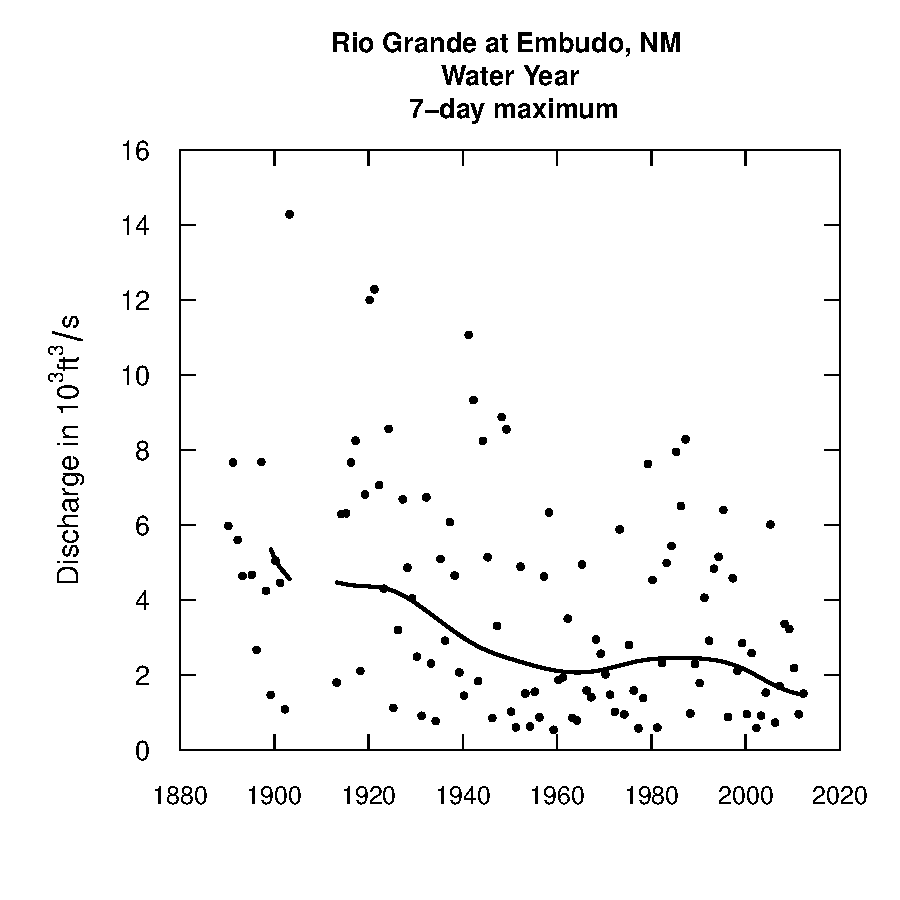
\includegraphics{EGRET-fig1}
\end{center}
\caption{7-day Maxiumum Flow (istat=7)}
\label{fig:plotflow}
\end{figure}

\FloatBarrier

%------------------------------------------------------------ 
\subsubsection{plotSDLogQ}
\label{sec:plotSDLogQ}
%------------------------------------------------------------ 
This function produces a graphic of the running standard deviation of the log of daily discharge over time.  The idea is to get some idea of how variability of daily discharge is changing over time.  By using the standard deviation of the log discharge the statistic becomes dimensionless.  It also means that it is a way of looking at variability quite aside from average values, so, in the case of a system where discharge might be increasing over a period of years, this provides a way of looking at the variability relative to that changing mean value.  It is much like a coefficient of variation, but it has sample properties that make it a smoother measure of variability.  There are often comments about how things like urbanization or enhanced greenhouse gases in the atmosphere are bringing about an increase in variability, this is one way to explore that idea.  In the simplest case the call is (Figure \ref{fig:SD1}):

\begin{Schunk}
\begin{Sinput}
> INFO <- setPA()
> plotSDLogQ()
\end{Sinput}
\end{Schunk}

If you were just interested in the variablility in spring (March-April-May), you could change paStart and paLong using the setPA function (Figure \ref{fig:SD2}). These figures show there is little change in variability on the Rio Grande between the water year and spring.  

\begin{Schunk}
\begin{Sinput}
> INFO <- setPA(paStart=3, paLong=3)
> plotSDLogQ()
\end{Sinput}
\end{Schunk}

\begin{figure}[htbp]
  \begin{minipage}[h]{0.5\linewidth}
    \begin{center}


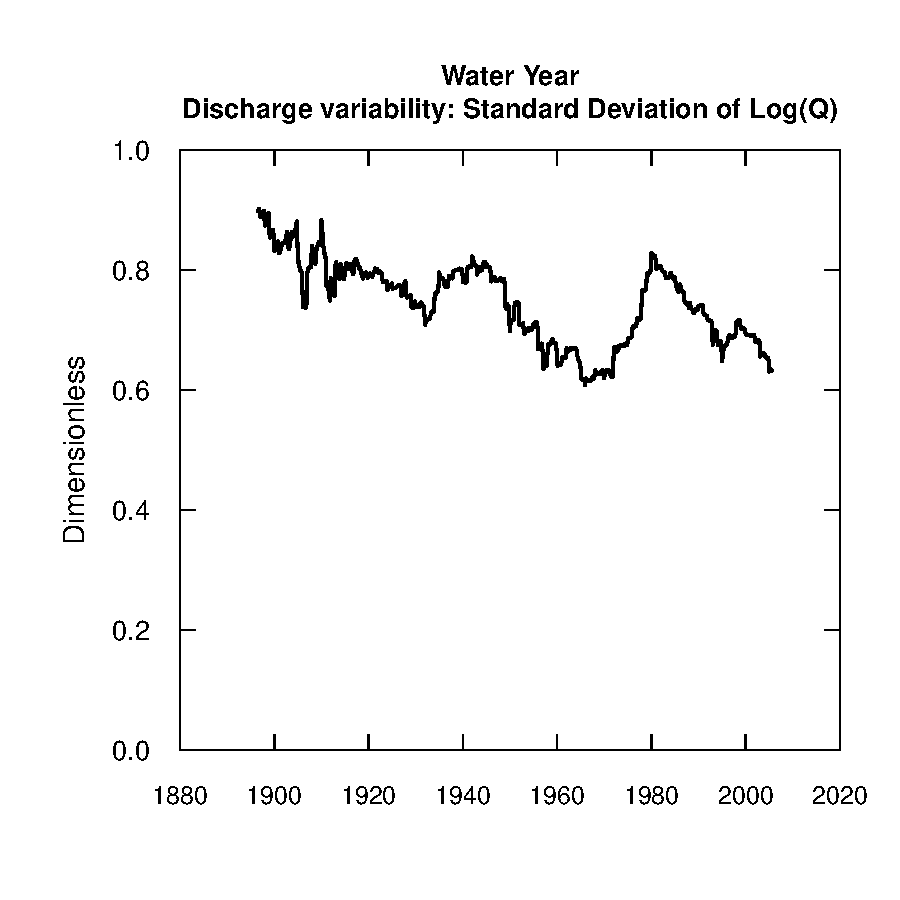
\includegraphics{EGRET-fig2a}
    \subcaption{Water Year}
    \label{fig:SD1}
    \end{center}
  \end{minipage}
  \hspace{0.5cm}
  \begin{minipage}[h]{0.5\linewidth}
    \begin{center}


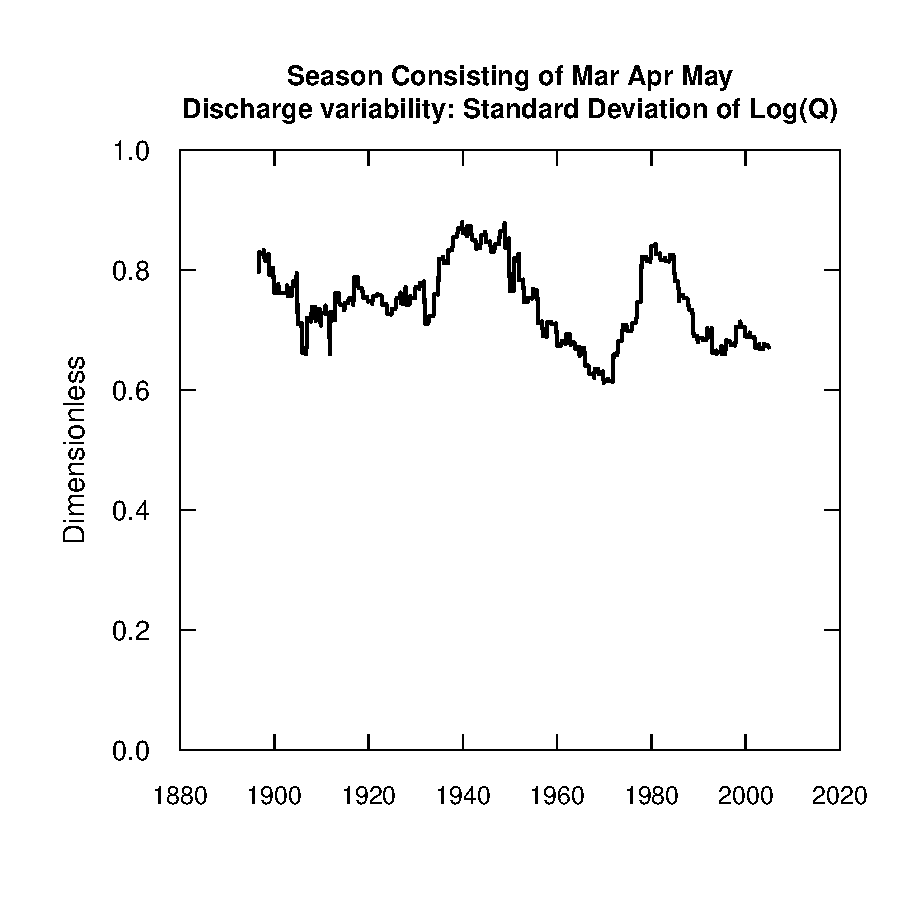
\includegraphics{EGRET-fig2b}
    \subcaption{Spring (March-May)}
    \label{fig:SD2}
    \end{center}
  \end{minipage}
  \caption{Discharge variability on the Rio Grande}
\end{figure}

A more interesting comparison might be between spring and summer on the Red River of the North (Figure \ref{fig:red}).  This figure shows that there is generally more variability in discharge in the spring compared to the summer.


\begin{figure}[htbp]
  \begin{minipage}[h]{0.5\linewidth}
    \begin{center}

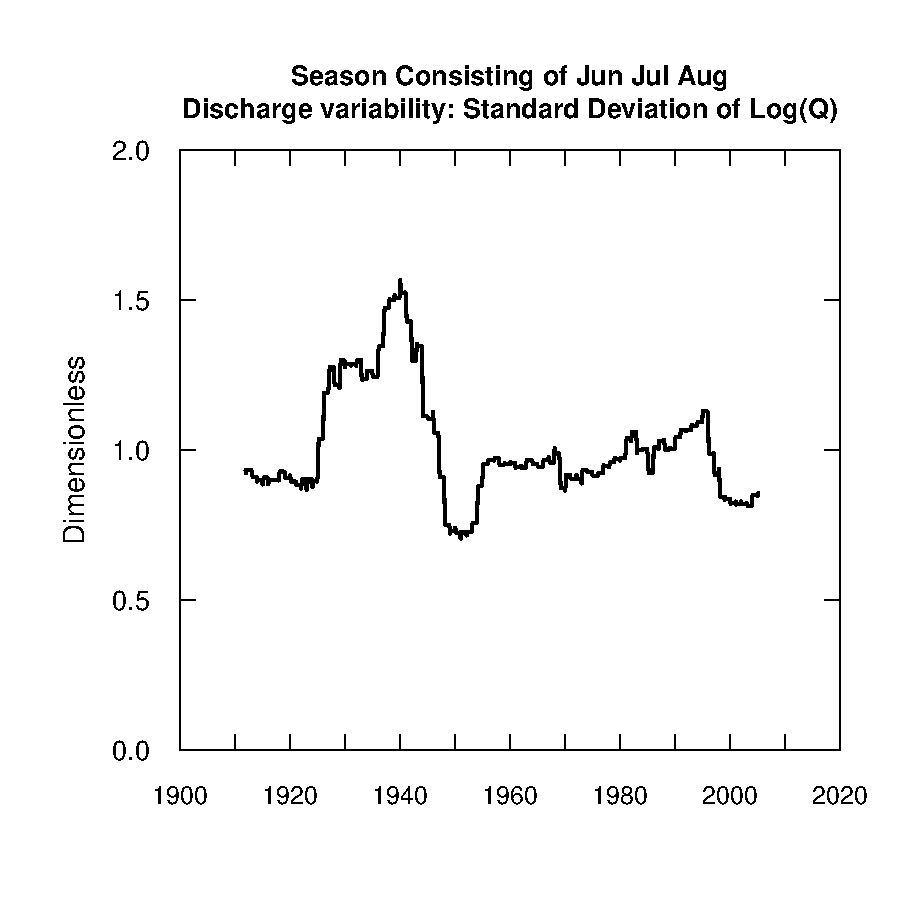
\includegraphics{EGRET-fig3a}
    \subcaption{Summer (June-August)}
    \label{fig:SDRed1}
    \end{center}
  \end{minipage}
  \hspace{0.5cm}
  \begin{minipage}[h]{0.5\linewidth}
    \begin{center}


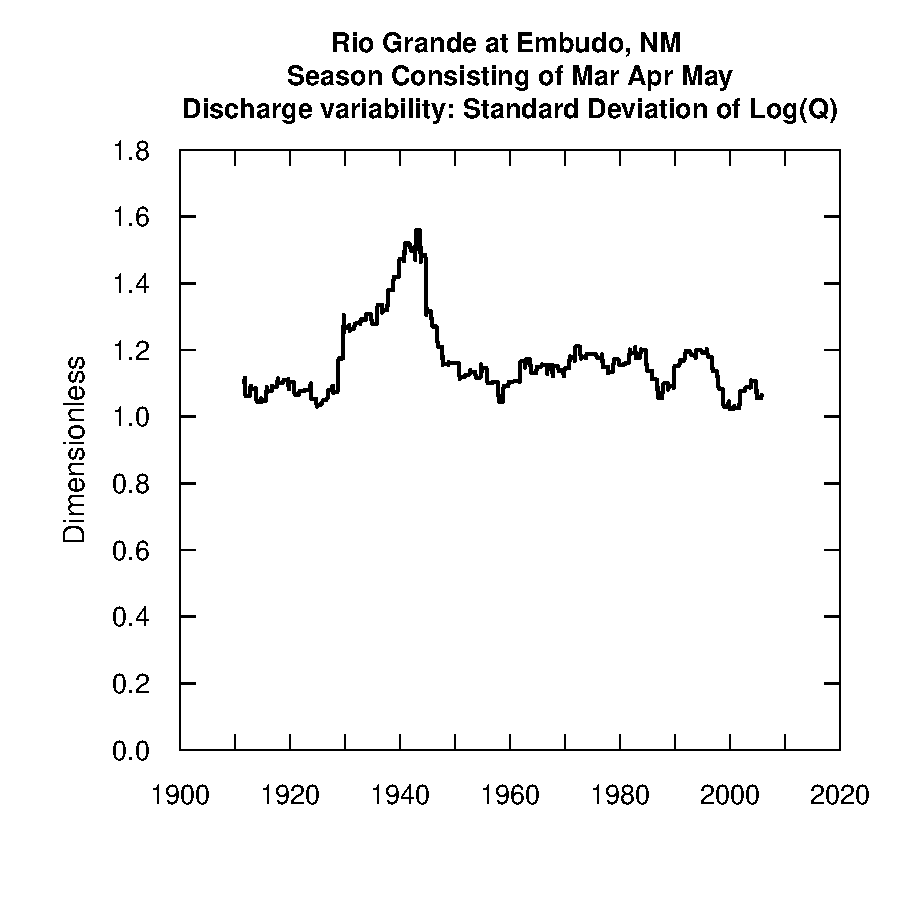
\includegraphics{EGRET-fig3b}
    \subcaption{Spring (March-May)}
    \label{fig:SDRed2}
    \end{center}
  \end{minipage}
  \caption{Discharge variability on the Red River of the North, ND}
  \label{fig:red}
\end{figure}

\FloatBarrier
%------------------------------------------------------------ 
\subsubsection{plotQTimeDaily}
\label{sec:plotQTimeDaily}
%------------------------------------------------------------ 
plotQTimeDaily is simply a time series plot of discharge.  But, it is most suited for showing events above some discharge threshold.  In the simplest case, it can plot the entire record, but given the line weight and use of an arithmetic scale it will primarily provide a visual focus on the higher values. plotQTimeDaily requires startYear and endYear, along with some other optional arguements (see ?plotQTimeDaily for more details).

Returning to our example concerning the Rio Grande (Figure \ref{fig:plotQTimeDaily}):
\begin{Schunk}
\begin{Sinput}
> plotQTimeDaily(1990,2000,qLower=2,qUnit=3)
\end{Sinput}
\end{Schunk}

\begin{figure}[h]
\begin{center}

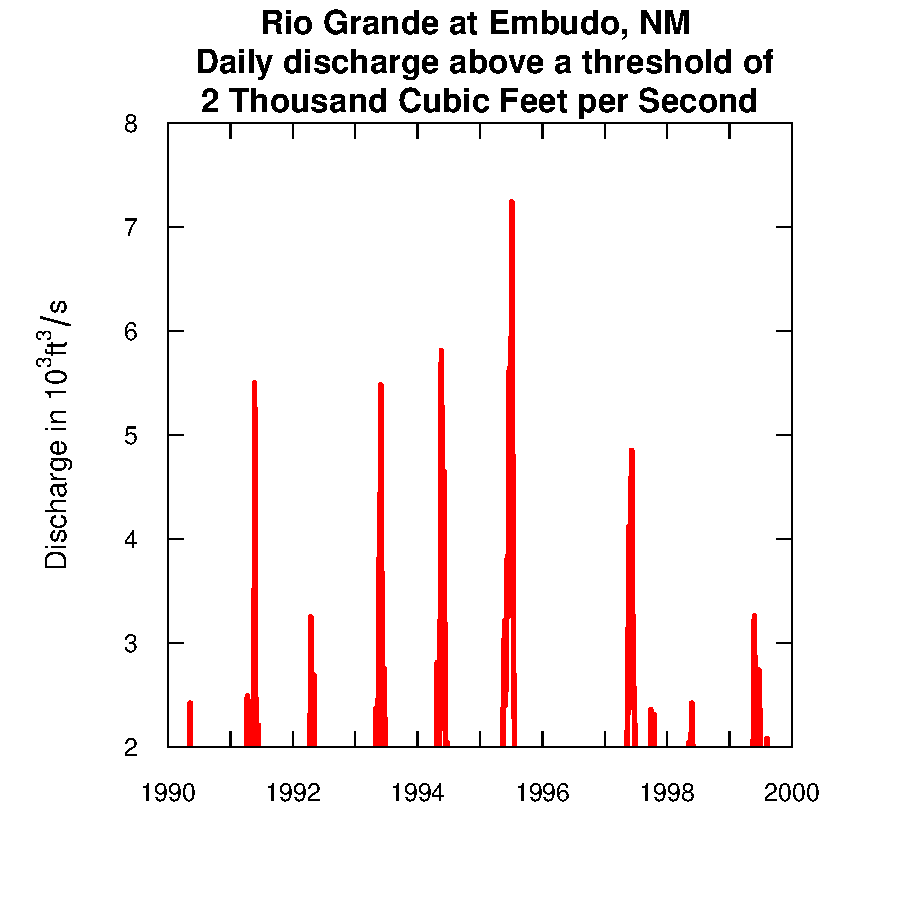
\includegraphics{EGRET-figplotQTimeDailyFig}
\end{center}
\caption{Discharge above a threshold}
\label{fig:plotQTimeDaily}
\end{figure}

\FloatBarrier
%------------------------------------------------------------ 
\subsubsection{plotFour}
\label{sec:plotFour}
%------------------------------------------------------------

\begin{Schunk}
\begin{Sinput}
> annualSeries <- makeAnnualSeries()
> plotFour(qUnit=3)
\end{Sinput}
\end{Schunk}

\begin{figure}[h]
\begin{center}

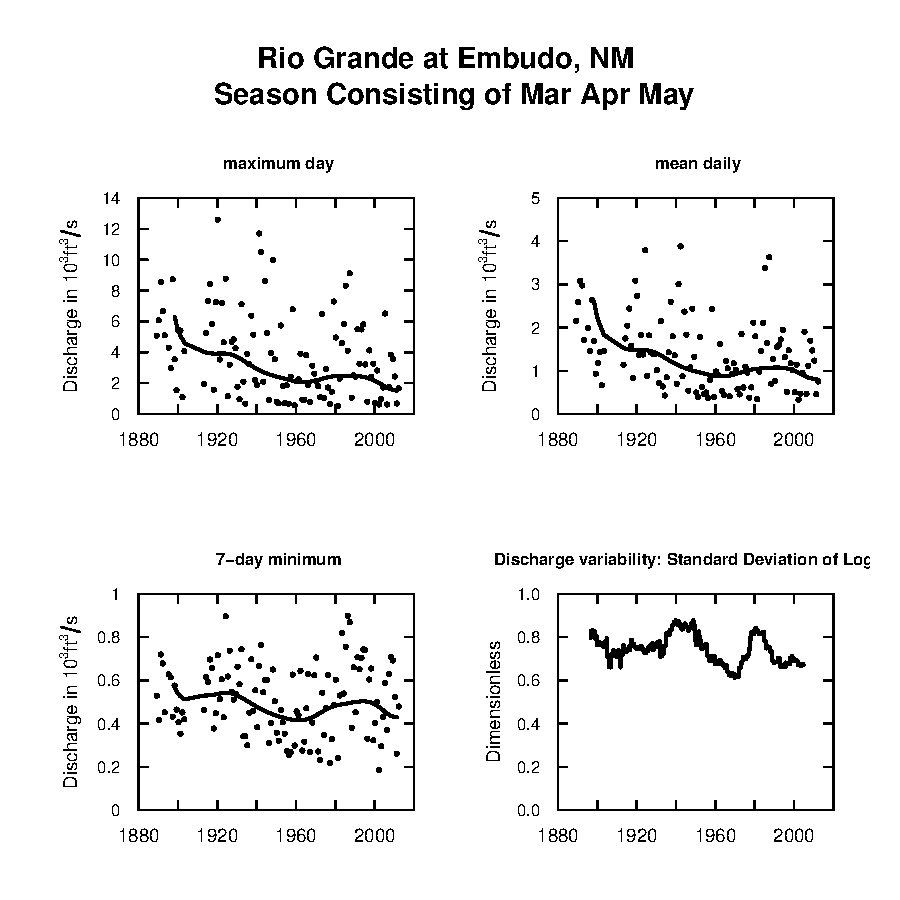
\includegraphics{EGRET-figplotFour}
\end{center}
\caption{Default plotFour}
\label{fig:plotFour}
\end{figure}

\FloatBarrier
%------------------------------------------------------------ 
\subsubsection{plotFourStats}
\label{plotFourStats}
%------------------------------------------------------------
\begin{Schunk}
\begin{Sinput}
> plotFourStats(qUnit=3)
\end{Sinput}
\end{Schunk}

\begin{figure}[h]
\begin{center}

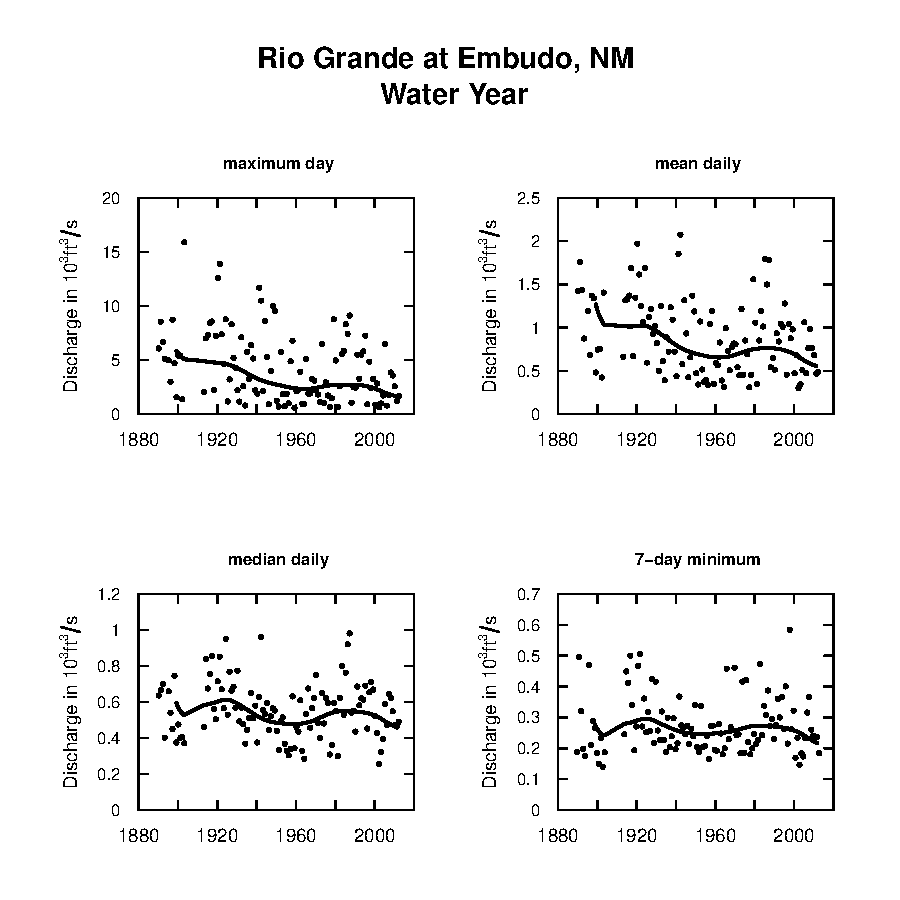
\includegraphics{EGRET-figplotFourStats}
\end{center}
\caption{Default plotFourStats}
\label{fig:plotFourStats}
\end{figure}

\FloatBarrier
%------------------------------------------------------------ 
\subsection{Table Options}
\label{sec:tableOptions}
%------------------------------------------------------------ 
Rathar than graphically, it is sometimes easier to consider the results in table formats. 

%------------------------------------------------------------ 
\subsubsection{printSeries}
\label{sec:printSeries}
%------------------------------------------------------------
Similar to the function plotFlowSingle, the printSeries will print the requested flow statistics (Table \ref{table:istat}). A small sample of the output is printed below.

\begin{Schunk}
\begin{Sinput}
> printSeries(istat=3, qUnit=3)
\end{Sinput}
\end{Schunk}

\begin{verbatim}
Rio Grande at Embudo, NM
 Water Year
    30-day minimum
    Thousand Cubic Feet per Second
   year   annual   smoothed
           value    value
   1899    0.280    0.296
   1900    0.208    0.285
   1901    0.169    0.277
   1902    0.320    0.272
...
   2011    0.252    0.248
   2012    0.257       NA
\end{verbatim}

\FloatBarrier
%------------------------------------------------------------ 
\subsubsection{tableFlowChange}
\label{sec:tableFlowChange}
%------------------------------------------------------------
Another way to look at the results is to consider how much the smoothed values change between various pairs of years.  These changes can be represented in four different ways.  
\begin{itemize}
  \item As a change between the first and last year of the pair, expressed in the flow units selected.
  \item As a change between the first and last year of the pair, expressed as a percentage of the value in the first year
  \item As a slope between the first and last year of the pair, expressed in terms of the flow units per year.
  \item As a slope between the first and last year of the pair, expressed as a percentage change per year (a percentage based on the value in the first year).
\end{itemize}

There is another argument that can be very useful in this function: yearPoints.  In the default case, the set of years that are compared are at 5 year intervals along the whole data set.  If the data set was quite long this can be a daunting number of comparisons.  For example, in an 80 year record, there would be 136 such pairs. Instead, we could look at changes for every 20 years starting in 1930: 

\begin{Schunk}
\begin{Sinput}
> tableFlowChange(istat=3, qUnit=3,yearPoints=c(1930,1950,1970,1990,2010))
\end{Sinput}
\begin{Soutput}
   Rio Grande at Embudo, NM
   Season Consisting of Mar Apr May
    30-day minimum 

             Streamflow Trends
   time span          change        slope       change        slope
                      10^3 cfs 10^3 cfs /yr         %         %/yr
 1930  to  1950       -0.089      -0.0045          -16         -0.8
 1930  to  1970         -0.1      -0.0025          -18        -0.45
 1930  to  1990       -0.046     -0.00077         -8.3        -0.14
 1930  to  2010        -0.11      -0.0013          -19        -0.24
 1950  to  1970       -0.011     -0.00054         -2.3        -0.12
 1950  to  1990        0.043       0.0011          9.2         0.23
 1950  to  2010       -0.016     -0.00026         -3.4       -0.056
 1970  to  1990        0.054       0.0027           12         0.59
 1970  to  2010      -0.0049     -0.00012         -1.1       -0.027
 1990  to  2010       -0.059      -0.0029          -12        -0.58
\end{Soutput}
\end{Schunk}


\FloatBarrier

%------------------------------------------------------------ 
\section{Water Quality Analysis (pre-WRTDS)}
\label{sec:wqa}
%------------------------------------------------------------ 
Before running the WRTDS model, it is very helpful to take a look at the measured data in a graphical way to understand its behavior and to identify things that might be errors in the data set or learn about the temporal distribution of the data (identify gaps) prior to running the model.  It is always best to clear up these issues before moving forward.

In this section and the next, we will use the Choptank River at Greensboro, MD as our example case. The Choptank River is a major tributary of the Chesapeake Bay. Inorganic nitrogen (nitrate and nitrite) has been measured from 1979. First, we need to get the streamflow and nitrate data into R, then use the mergeReport function to associate flow with the discrete measured water quality data.


\begin{Schunk}
\begin{Sinput}
> siteID <- "01491000" #Choptank River at Greensboro, MD
> startDate <- "1979-10-01"
> endDate <- "2011-09-30"
> param<-"00631"
> INFO<- getMetaData(siteID,param,interactive=FALSE)
> INFO$shortName <- "Choptank River"
> Sample <- getSampleData(siteID,param,startDate,endDate)
> Sample <- mergeReport()
\end{Sinput}
\end{Schunk}

%------------------------------------------------------------ 
\subsection{Water Quality Plotting Variables}
\label{sec:wqVariables}
%------------------------------------------------------------
The next section will cover the available plots in the EGRET package. This section will briefly summarize common input variables (arguments) for those functions.

\begin{table}
\caption{Variables used in water quality analysis plots  \label{tab:wqVariables}}
\begin{tabularx}{\textwidth}{lX}
\hline
  \textbf{Argument} & \textbf{Definition} \\
\hline
qUnit & Determines what units will be used for discharge, see \ref{sec:units}\\
printTitle & If TRUE the plot has a title.  If FALSE no title (useful for publications where there will be a caption)\\
qLower & The lower bound on the discharge on the day of sampling that will be used in forming a subset of the sample data set that will be displayed in the graph.  It is expressed in the units specified in qUnit.  If qLower = NA, then the lower bound is set to zero.\\
qUpper & The upper bound on the discharge on the day of sampling that will be used in forming a subset of the sample data set that will be displayed in the graph.  It is expressed in the units specified in qUnit.  If qUpper = NA, then the lower bound is set to infinity.\\
paLong & The length of the time period that will be used in forming a subset of the sample data set that will be displayed in the graph, expressed in months. \\ 
paStart & The starting month for the time period that will be used in forming a subset of the sample data set that will be displayed in the graph.  It is expressed in months (calendar months).\\
concMax & The upper limit on the vertical axis of graphs showing concentration values in mg/L (NA sets value to just above maximum).  \\
concMin & The lower limit on the vertical axis of graphs showing concentration values in mg/L (NA sets value to just below minimum for log scales, zero for linear).  \\
fluxUnit & Determines what units will be used for flux (see Section \ref{sec:units}).\\
fluxMax & The upper limit on the vertical axis of graphs showing flux values.  \\
\hline
\end{tabularx}

\end{table}

%------------------------------------------------------------ 
\subsection{Water Quality Plots}
\label{sec:wqPlots}
%------------------------------------------------------------

%------------------------------------------------------------ 
\section{WRTDS Analysis}
\label{sec:wrtds}
%------------------------------------------------------------ 
Weighted Regressions on Time, Discharge and Season (WRTDS) creates a model of long-term trends in river-water quality, seasonal components, and discharge-related components of the behavior of measured water-quality parameters. In this section, we will step though the process require for a WRTDS analysis. The following section (\ref{sec:wrtdsResults}) will detail the available methods to view and evaluate the model results.


\begin{Schunk}
\begin{Sinput}
> modelEstimation()
> AnnualResults<-setupYears()
\end{Sinput}
\end{Schunk}


%------------------------------------------------------------ 
\section{WRTDS Results}
\label{sec:wrtdsResults}
%------------------------------------------------------------ 


\newpage
\appendix
%------------------------------------------------------------ 
\section{Appendix 1: Getting Started}
\label{sec:appendix1}
%------------------------------------------------------------ 
This section describes the options for downloading and installing the dataRetrieval package.

%------------------------------------------------------------
\subsection{New to R?}
%------------------------------------------------------------ 
If you are new to R, you will need to first install the latest version of R, which can be found here: \url{http://www.r-project.org/}.

There are many options for running and editing R code, one nice environment to learn R is RStudio. RStudio can be downloaded here: \url{http://rstudio.org/}. Once R and RStudio are installed, the environment package needs to be installed as described in the next section.

At any time, you can get information about any function in R by typing a question mark before the functions name.  This will open a file (in RStudio, in the Help window) that describes the function, the required arguments, and provides working examples.

\begin{Schunk}
\begin{Sinput}
> ?getJulian
\end{Sinput}
\end{Schunk}

To see the raw code for a particular code, type the name of the function:
\begin{Schunk}
\begin{Sinput}
> getJulian
\end{Sinput}
\begin{Soutput}
function(date) {
  # enter date in quotes for example "1949-09-30" 
  # program returns the julian date  
  dateTime <- as.Date(date)
  Julian <- as.numeric(julian(dateTime, origin = as.Date("1850-01-01")))
  return(Julian)
}
<environment: namespace:EGRET>
\end{Soutput}
\end{Schunk}


%------------------------------------------------------------
\subsection{R User: Installing EGRET}
%------------------------------------------------------------ 
To install the EGRET packages and it's dependencies:

\begin{Schunk}
\begin{Sinput}
> install.packages(c("zoo","survival","methods","fields","spam"))
> install.packages("dataRetrieval", repos="http://usgs-r.github.com/EGRET/", 
                  type="source")
> install.packages("EGRET", repos="http://usgs-r.github.com/EGRET/", 
                  type="source")
\end{Sinput}
\end{Schunk}

It is a good idea to re-start the R enviornment after installing the package, especially if installing an updated version (that is, restart RStudio). Some users have found it necessary to delete the previous version's package folder before installing newer version of EGRET. If you are experiencing issues after updating a package, trying deleting the package folder - the default location for Windows is something like this: C:/Users/userA/Documents/R/win-library/2.15/EGRET, and the default for a Mac: /Users/userA/Library/R/2.15/library/EGRET. Then, re-install the package using the directions above. Moving to CRAN should solve this problem.

After installing the package, you need to open the library each time you re-start R.  This is done with the simple command:
\begin{Schunk}
\begin{Sinput}
> library(dataRetrieval)
> library(EGRET)
\end{Sinput}
\end{Schunk}
Using RStudio, you could alternatively click on the checkbox for dataRetrieval and EGRET in the Packages window.

%------------------------------------------------------------
\subsection{R Developers: Installing EGRET from gitHub}
%------------------------------------------------------------
Alternatively, R-developers can install the most recent (not-necessarily stable) version of EGRET directly from gitHub using the devtools package.  devtools is available on CRAN.  Simply type the following commands into R to install the latest version of EGRET available on gitHub.  Rtools (for Windows) and appropriate \LaTeX\ tools are required. Be aware that the version installed using this method isn't necessarily the same as the version in the stable release branch.  


\begin{Schunk}
\begin{Sinput}
> library(devtools)
> install_github("dataRetrieval", "USGS-R")
> install_github("EGRET", "USGS-R")
\end{Sinput}
\end{Schunk}
To then open the library, simply type:

\begin{Schunk}
\begin{Sinput}
> library(dataRetrieval)
> library(EGRET)
\end{Sinput}
\end{Schunk}


%------------------------------------------------------------
% BIBLIO
%------------------------------------------------------------
\begin{thebibliography}{10}

\bibitem{HirschI}
Helsel, D.R. and R. M. Hirsch, 2002. Statistical Methods in Water Resources Techniques of Water Resources Investigations, Book 4, chapter A3. U.S. Geological Survey. 522 pages. \url{http://pubs.usgs.gov/twri/twri4a3/}

\bibitem{HirschII}
Hirsch, R. M., Moyer, D. L. and Archfield, S. A. (2010), Weighted Regressions on Time, Discharge, and Season (WRTDS), with an Application to Chesapeake Bay River Inputs. JAWRA Journal of the American Water Resources Association, 46: 857-880. doi: 10.1111/j.1752-1688.2010.00482.x \url{http://onlinelibrary.wiley.com/doi/10.1111/j.1752-1688.2010.00482.x/full}

\bibitem{HirschIII}
Sprague, L. A., Hirsch, R. M., and Aulenbach, B. T. (2011), Nitrate in the Mississippi River and Its Tributaries, 1980 to 2008: Are We Making Progress? Environmental Science \& Technology, 45 (17): 7209-7216. doi: 10.1021/es201221s \url{http://pubs.acs.org/doi/abs/10.1021/es201221s}

\end{thebibliography}

\end{document}

\end{document}
